\documentclass[10pt]{beamer}
\usetheme{CambridgeUS}
\usepackage[utf8]{inputenc}
\usepackage[spanish]{babel}
\usepackage{amsmath}
\usepackage{amsfonts}
\usepackage{amssymb}
\usepackage{graphicx}
\usepackage{ragged2e}
\usepackage{multicol}
\usepackage{multirow, array}
\author{Kevin García - Alejandro Vargas}
\title{Réplica libro: Zero Acceptance Number Sampling Plans Squeglia (2008)}
%\setbeamercovered{transparent} 
%\setbeamertemplate{navigation symbols}{} 
%\logo{} 
%\institute{} 
%\date{} 
%\subject{} 
\justifying
\begin{document}

\begin{frame}[plain]
\maketitle
\end{frame}

\begin{frame}{Contenido}
\tableofcontents
\end{frame}

\section{Introducción}
\begin{frame}{Introducción}
Squeglia (2008)\cite{A0} nos muestra en su libro una comparación bastante completa entre el muestreo de aceptación y rechazo para atributos por el método MIL-STD-105E/ANSI Z1.4 y los planes de muestreo c=0, dichas comparaciones se realizan en términos de tamaños de muestra, curvas características de operación y del AOQL (Máximo porcentaje de defectuosos esperado). En esta presentación se tratará de replicar algunos de los resultados y comparaciones obtenidos por Squeglia. Para que este sea legible, se darán unos conceptos introductorios y se contextualizará al público acerca del funcionamiento de estos dos planes de muestreo de aceptación.
\end{frame}

\subsection{Conceptos previos}
\begin{frame}{Introducción}
Algunos conceptos claves, que se mencionarán de aquí en adelante son:
\begin{itemize}
\item AQL (aceptable quality level). Representa el más pobre nivel de calidad del proceso del proveedor que el consumidor considera aceptable como un proceso promedio. La probabilidad de aceptar este nivel de calidad debe ser alta y se denota por $(1-\alpha)$, donde $\alpha$ es el riesgo del productor.
\item LTPD (lot tolerance percent defective). Es el peor nivel de calidad que el consumidor esta dispuesto a aceptar en un lote individual. También se le conoce como nivel de calidad rechazable(RQL) y se denota por $\beta$(riesgo de consumidor).
\end{itemize}
El AQL describe lo que el plan de muestreo aceptará y el LTPD describe lo que el plan de muestreo rechazará. Se desea designar un plan de muestreo que acepte un lote de producto particular en el AQL la mayoría de las veces y que lo rechace en el RQL la mayor parte del tiempo.
\end{frame}

\begin{frame}{Introducción}
\begin{itemize}
\item Curva Característica de Operación (OC). Mide el desempeño del plan de muestreo de aceptación. Da la probabilidad de aceptar un lote dependiendo del tamaño del lote, de la proporción de defectuosos en el lote,del tamaño de la muestra y del número de aceptación.
\item AOQ: Calidad Promedio de Salida. Proporción promedio de unidades defectuosas entre aquellas unidades que superan el proceso de inspección. (Este concepto es una forma de medir el efecto de un plan de muestreo sobre la calidad que se tendrá después de aplicarlo). Se calcula como $AOQ=P_a*P$, donde $P_a$ es la probabilidad de aceptación y $P$ es la proporción real de defectuosos.
\item AOQL: Máxima Calidad Promedio de Salida. Se calcula como $Max(AOQ)$
\end{itemize}
\end{frame}

\section{MIL-STD-105E/ANSI Z1.4}
\begin{frame}{MIL-STD-105E/ANSI Z1.4}
La norma MIL-STD-105E es un esquema de muestreo que ideó el gobierno de Estados Unidos para sus adquisiciones durante la Segunda Guerra Mundial. MIL-STD-105E está diseñada para muestreo de atributos lote por lote. Se usa AQL entre 0,10 a 10\%. Para utilizar un plan de muestreo indexado según AQL como la norma MIL-STD-105E se deben seguir los siguientes pasos:
\begin{itemize}
\item[1.] Establecer el valor de AQL.
\item[2.] Determinar el tamaño del lote N.
\item[3.] Determinar el nivel de inspección: generalmente inspección nivel II (normal).
\item[4.] Determinar el plan de muestreo: muestreo sencillo, doble o múltiple.
\item[5.] Determinar la clave de tamaño de muestra (letra)
\item[6.] Determinar el tamaño de muestra y el número de aceptación
\item[7.] Seleccionar la muestra: se debe tomar del lote al azar.
\item[8.] Inspeccionar la muestra: se cuentan los artículos defectuosos. Si el número que resulta no supera el número de aceptación que se encontró en la tabla se acepta el lote. En caso contrario se rechaza.
\end{itemize}
\end{frame}

\section{Planes de muestreo c=0}
\begin{frame}{Planes de muestreo c=0}
Los planes ``Aceptar en ninguno'', comúnmente llamados planes C = 0, son planes de muestreo de lotes para datos de atributos diseñados de tal manera que si se encuentra un defecto en la muestra inspeccionada, el lote se rechaza. El tamaño de muestra se puede encontrar directamente con la fórmula
$$n=\frac{ln(\beta)}{ln(1-LTPD)}$$ 
donde se deben determinar valores para $\beta$(usualmente 0.1) y $LTPD$ mencionados en la introducción. Se procede igual que en el método anterior, pero en este caso, si el número de defectuosos es mayor o igual a 1, se rechaza el lote.
\end{frame}


\section{Comparación y resultados}
\begin{frame}{Resultados}
Mientras el ANSI (MIL-STD-105) es un sistema AQL (protege al productor - Si la calidad está en el AQL, nos aseguramos de que se pueda aceptar el lote), C = 0 es un sistema LTPD (protege al consumidor - si la calidad está en el LTPD nos permite asegurarnos de que rechazamos).

~\\Lo primero que trata de mostrar Squeglia en su libro, son los efectos de los números de aceptación en la curva OC, para ello compara dos planes de muestreo, uno con un tamaño de muestra $n=125$ y un número de aceptación $c=10$, y el otro con un tamaño de muestra $n=18$ y un número de aceptación $c=0$.

~\\``\textit{Con el número de aceptación establecido en cero, tenemos una mayor protección en el nivel LTPD con un tamaño de muestra de 18, en comparación con un plan de muestreo de ANSI Z1.4 que tiene un tamaño de muestra de 125 con un número de aceptación de 10}''
\end{frame}

\begin{frame}{Resultados}
\begin{figure}[h!]
  \centering
  \includegraphics[scale=0.33]{FigurasUV/Figura2.pdf}
  \caption{Efecto del número de aceptación en la curva característica de operación}
\end{figure}
\end{frame}

\begin{frame}{Resultados}
Otro aspecto importante que se compara en este libro, es el tamaño de muestra necesario para dos niveles de AQL establecidos, en la tabla 1 se observa la comparación que obtuvimos con la ayuda del paquete \cite{AyR} para el ANSI Z1.4 y con código propio para los planes c=0, y además, le añadimos los riesgos del productor que se podrían dar con cada uno de los planes de muestreo.

\begin{table}[htbp]
  \centering
    \begin{tabular}{c|c|c|c|c}
    \hline
    \textbf{Método} & \textbf{AQL} & \textbf{n} & \textbf{c} & \textbf{$\alpha$} \\
    \hline
    \multirow{2}[2]{*}{\textbf{ANSI Z1.4}} & 0.01  & 125   & 3     & 0.03745 \\
          & 0.04  & 125   & 10    & 0.01191 \\
    \hline
    \multirow{2}[2]{*}{\textbf{Planes C=0}} & 0.01  & 42    & 0     & 0.34434 \\
          & 0.04  & 18    & 0     & 0.52040 \\
    \hline
    \end{tabular}%
    \caption{Comparación tamaños de muestra ambos planes}
  \label{tab:addlabel}%
\end{table}%
Se observa que se realiza menos inspección (el tamaño de muestra es considerablemente inferior para valor de AQL mayores). 
\end{frame}

\begin{frame}{Resultados}
Otro aspecto importante que menciona Squeglia es el concepto del AOQL, él lo define como el máximo promedio de calidad saliente de una estación de inspección para un plan de muestreo en particular. Squeglia ejemplifica esto mostrando una curva AOQ para el plan de muestreo $n=50$ y $c=0$, el AOQL se encuentra en el punto máximo de esta curva. En la figura 2 se pueden observar los resultados replicados. De esta gráfica podemos decir que no importa qué tan mala sea la proporción de defectuosos en los lotes que entran, la calidad promedio de salida nunca será peor que 0.73\% de defectuosos en promedio.
\end{frame}

\begin{frame}{Resultados}
\begin{figure}[h!]
  \centering
  \includegraphics[scale=0.34]{FigurasUV/Figura3.pdf}
  \caption{Curva AOQL}
\end{figure}
\end{frame}

\begin{frame}{Resultados}
En la figura 3 se muestra una comparación de los valores de AOQL para varios tamaños de muestra y números de aceptación. Al igual que el autor, utilizamos infinitos tamaños de lote para construir este gráfico. Se puede apreciar que mientras mayor sea el tamaño de muestra \textbf{n}, y menor sea el número de aceptación \textbf{c}, el AOQL(máxima calidad promedio de salida) es menor, es decir, la calidad promedio de salida en el peor de los casos, va a presentar un porcentaje mucho menor de productos defectuosos.
\end{frame}

\begin{frame}{Resultados}
\begin{figure}[h!]
  \centering
  \includegraphics[scale=0.33]{FigurasUV/Figura4.pdf}
  \caption{Curvas para determinar valores AOQL}
\end{figure}
\end{frame}

\begin{frame}{Resultados}
\begin{table}[htbp]
  \centering
    \begin{tabular}{|c|c|c|}
    \hline
    \multicolumn{1}{|c|}{\multirow{2}[4]{*}{\textbf{Número de\newline{} aceptación c}}} & \multicolumn{2}{c|}{\textbf{Tamaño de muestra n}} \\
\cline{2-3}          & \textbf{20} & \textbf{80} \\
    \hline
    \textbf{0} & 0.0437 & 0.0108 \\
    \hline
    \textbf{1} & 0.072 & 0.0174 \\
    \hline
    \end{tabular}%
    \caption{AOQL por tamaño de muestra y número de aceptación}
  \label{tab:addlabel}%
\end{table}%
\end{frame}

\begin{frame}{Resultados}
\begin{figure}[h!]
  \centering
  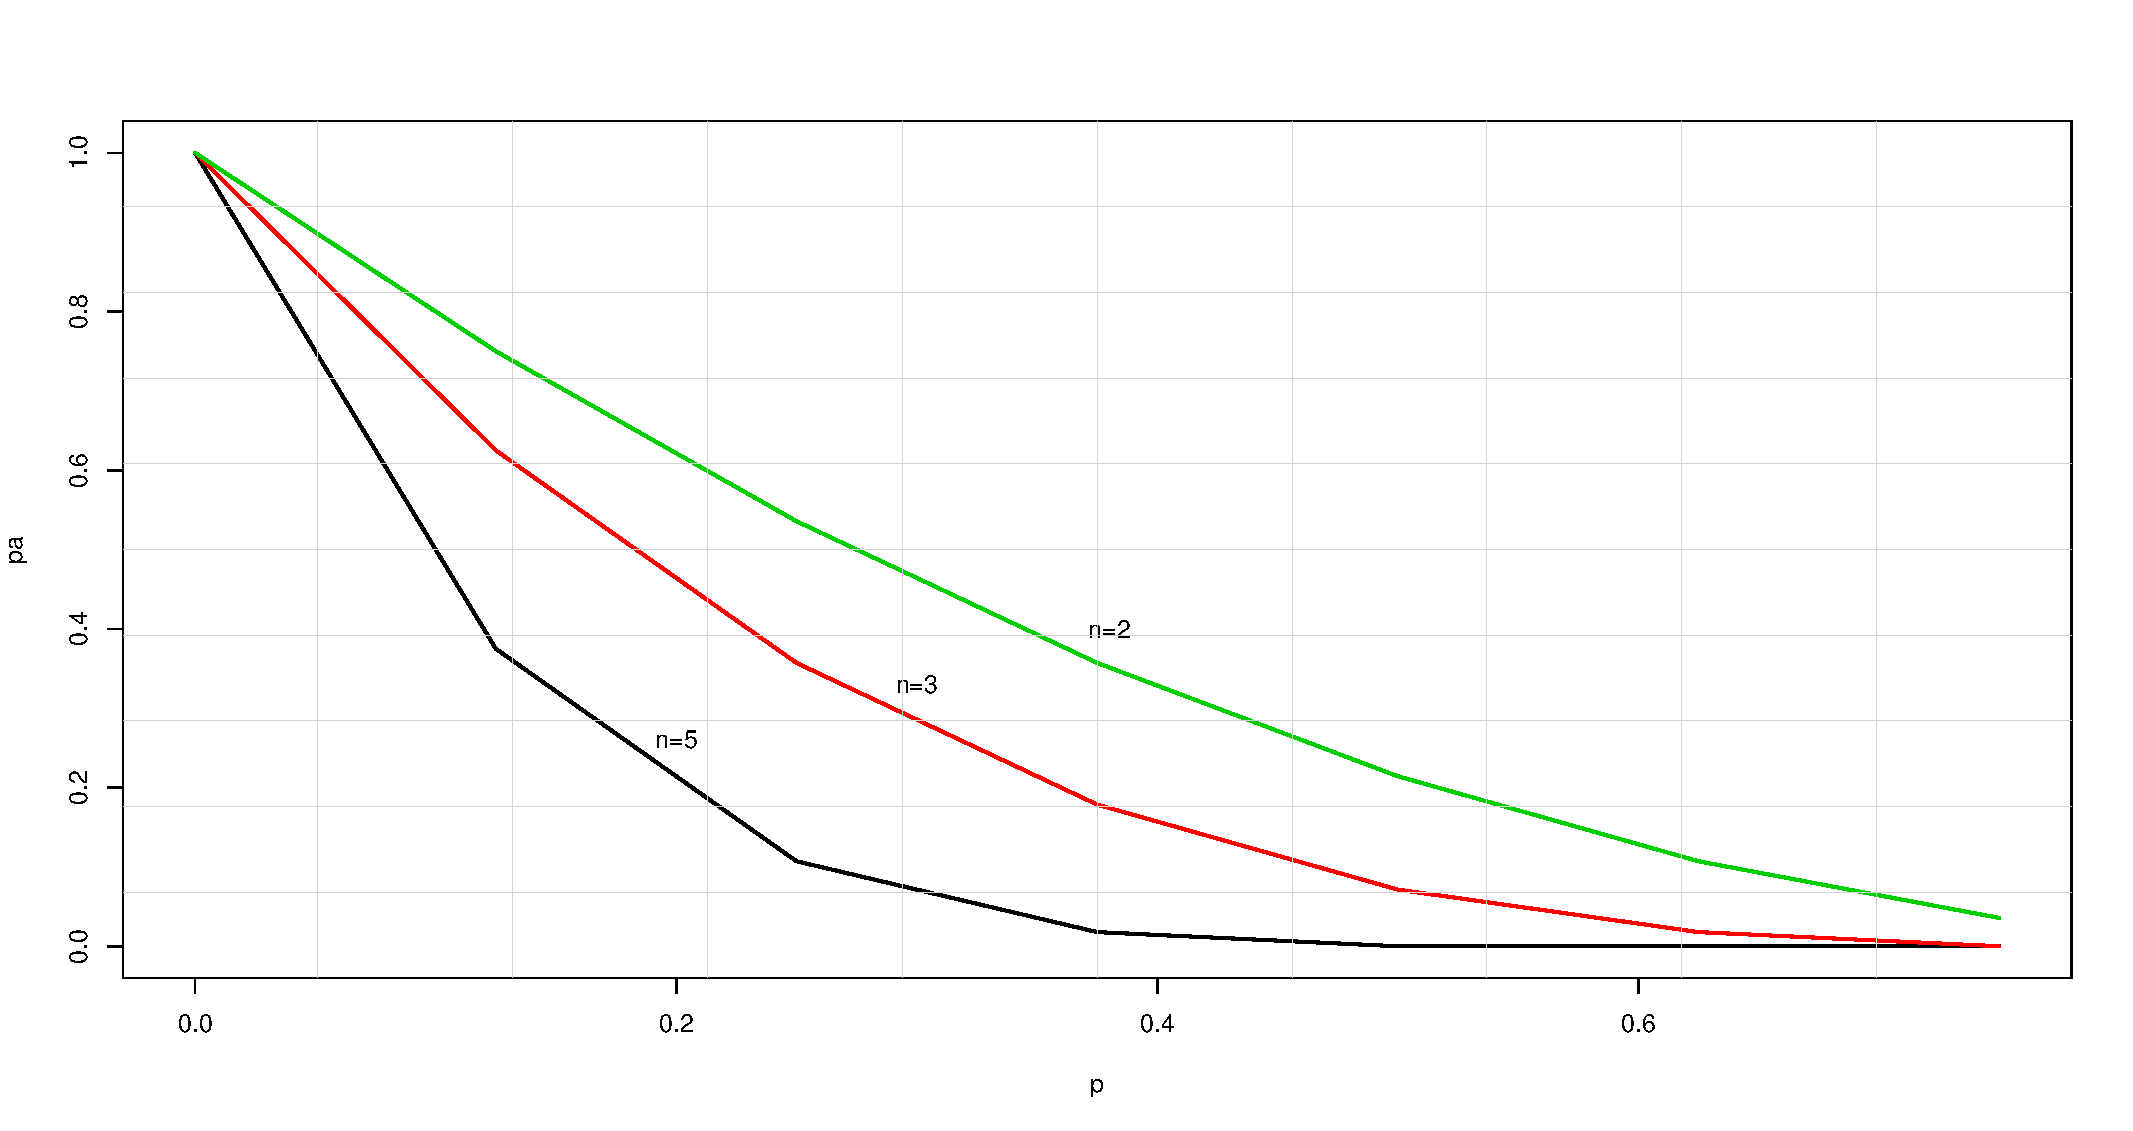
\includegraphics[scale=0.33]{FigurasUV/CO1.pdf}
  \caption{Curvas OC para planes de muestreo simples con C=0. Tamaño del lote 2 - 8}
\end{figure}
\end{frame}

\begin{frame}{Resultados}
\begin{figure}[h!]
  \centering
  \includegraphics[scale=0.33]{FigurasUV/CO8.pdf}
  \caption{Curvas OC para planes de muestreo simples con C=0. Tamaño del lote 281 - 500}
\end{figure}
\end{frame}

\begin{frame}{Resultados}
\begin{figure}[h!]
  \centering
  \includegraphics[scale=0.33]{FigurasUV/CO14.pdf}
  \caption{Curvas OC para planes de muestreo simples con C=0. Tamaño del lote 150001 - 500000}
\end{figure}
\end{frame}


\section{Conclusiones}
\begin{frame}{Conclusiones}
Algunas conclusiones importantes que se obtienen, a partir de los resultados nuestros y del libro de Squeglia comparando ambos métodos de muestreo(MIL-STD-105E/ANSI Z1.4 y C=0) de aceptación son:
\begin{itemize}
\item[1.]Los planes de aceptación cero desarrollados por Squeglia están diseñados ``para brindar una protección general al consumidor igual o mayor con menos inspección que los planes de muestreo MIL-STD-105 correspondientes''. Como se pudo observar en las probabilidades de aceptación, para lotes con niveles de defectos reales mayores que 0 pero menores que el RQL, es más probable que el enfoque C = 0 rechace el lote (proteja al consumidor).

\item[2.]Si la calidad está cerca del 100\%, los planes C = 0 darán como resultado que se inspeccionen menos partes en total.

\item[3.]Los planes C=0 pueden afectar considerablemente al productor, ya que, si la calidad no está cerca del 100\%, los planes C = 0 darán como resultado más lotes rechazados. Un plan estándar(ANSI Z1.4) teóricamente aceptaría un lote con el nivel de AQL de defectos el 95\% del tiempo, mientras que el plan C = 0 rechazaría con mucha mayor frecuencia.
\end{itemize}
\end{frame}


\section{Bibliografía}
\begin{frame}
  \frametitle{Bibliografía}
  
\nocite{A0,ControlR}
  
  \bibliographystyle{plain}
  \bibliography{references}
\end{frame}

\section{Anexos}
\begin{frame}{Anexos}
\begin{figure}[h!]
  \centering
  \includegraphics[scale=0.55]{FigurasUV/letra.png}
  \caption{Letra código del plan}
\end{figure}
\end{frame}

\begin{frame}{Anexos}
\begin{figure}[h!]
  \centering
  \includegraphics[scale=0.6]{FigurasUV/n.png}
  \caption{Tamaño de muestra}
\end{figure}
\end{frame}

\begin{frame}{Anexos}
\begin{figure}[h!]
  \centering
  \includegraphics[scale=0.33]{FigurasUV/CO2.pdf}
  \caption{Curvas OC para planes de muestreo simples con C=0. Tamaño del lote 9 - 15}
\end{figure}
\end{frame}

\begin{frame}{Anexos}
\begin{figure}[h!]
  \centering
  \includegraphics[scale=0.33]{FigurasUV/CO3.pdf}
  \caption{Curvas OC para planes de muestreo simples con C=0. Tamaño del lote 16 - 25}
\end{figure}
\end{frame}

\begin{frame}{Anexos}
\begin{figure}[h!]
  \centering
  \includegraphics[scale=0.33]{FigurasUV/CO4.pdf}
  \caption{Curvas OC para planes de muestreo simples con C=0. Tamaño del lote 26 - 50}
\end{figure}
\end{frame}

\begin{frame}{Anexos}
\begin{figure}[h!]
  \centering
  \includegraphics[scale=0.33]{FigurasUV/CO5.pdf}
  \caption{Curvas OC para planes de muestreo simples con C=0. Tamaño del lote 51 - 90}
\end{figure}
\end{frame}

\begin{frame}{Anexos}
\begin{figure}[h!]
  \centering
  \includegraphics[scale=0.33]{FigurasUV/CO6.pdf}
  \caption{Curvas OC para planes de muestreo simples con C=0. Tamaño del lote 91 - 150}
\end{figure}
\end{frame}

\begin{frame}{Anexos}
\begin{figure}[h!]
  \centering
  \includegraphics[scale=0.33]{FigurasUV/CO7.pdf}
  \caption{Curvas OC para planes de muestreo simples con C=0. Tamaño del lote 151 - 280}
\end{figure}
\end{frame}

\begin{frame}{Anexos}
\begin{figure}[h!]
  \centering
  \includegraphics[scale=0.33]{FigurasUV/CO9.pdf}
  \caption{Curvas OC para planes de muestreo simples con C=0. Tamaño del lote 501 - 1200}
\end{figure}
\end{frame}

\begin{frame}{Anexos}
\begin{figure}[h!]
  \centering
  \includegraphics[scale=0.33]{FigurasUV/CO10.pdf}
  \caption{Curvas OC para planes de muestreo simples con C=0. Tamaño del lote 1201 - 3200}
\end{figure}
\end{frame}

\begin{frame}{Anexos}
\begin{figure}[h!]
  \centering
  \includegraphics[scale=0.33]{FigurasUV/CO11.pdf}
  \caption{Curvas OC para planes de muestreo simples con C=0. Tamaño del lote 3201 - 10000}
\end{figure}
\end{frame}

\begin{frame}{Anexos}
\begin{figure}[h!]
  \centering
  \includegraphics[scale=0.33]{FigurasUV/CO12.pdf}
  \caption{Curvas OC para planes de muestreo simples con C=0. Tamaño del lote 10001 - 35000}
\end{figure}
\end{frame}

\begin{frame}{Anexos}
\begin{figure}[h!]
  \centering
  \includegraphics[scale=0.33]{FigurasUV/CO13.pdf}
  \caption{Curvas OC para planes de muestreo simples con C=0. Tamaño del lote 35001 - 150000}
\end{figure}
\end{frame}
\end{document}
